\capitulo{3}{Conceptos teóricos}

En este apartado, se van a exponer aquellos conceptos que requieran ser conocidos para comprender cómo se ha realizado el TFG.

\section{Procesamiento de vídeo}
Dado que este proyecto se fundamenta en obtener datos a partir de vídeos, es necesario conocer algunos conceptos básicos de procesamiento de vídeo.

\subsection{Vídeos}
Para que los vídeos sean procesados, es necesario que exista un proceso de lectura de los fotogramas. Además, en ocasiones se desea que los fotogramas sean guardados con el procesado realizado. Esto es lo que se conoce como objetos de vídeo. Un objeto de vídeo puede ser de lectura, cuando se pretende leer los fotogramas del vídeo, o de escritura, cuando se pretende guardar imágenes en forma de vídeo.

Leer un vídeo no requiere un mayor conocimiento más allá de conocer el concepto de fotograma, pero a la hora de escribir un vídeo es necesario conocer el concepto de codificación. Cuando se desea guardar un vídeo o una colección de fotogramas, se puede codificar en varios tipos, lo cual afectará al tipo de extensión del vídeo. Los codificadores más comunes son: MPEG, H.264, MJPEG, Sorenson, WMV, Ogg Theora, DivX y XviD.

Dependiendo del uso que se le vaya a dar al vídeo, conviene utilizar una codificación u otra, dando lugar a extensiones de vídeo diferentes. Estas extensiones definen el tipo de formato del vídeo. Los más comunes son: AVI, MOV, MP4, ASF, OGG, FLV, MKV y VOB.

Los vídeos están formados por varias imágenes consecutivas capturadas y reproducidas a cierta velocidad. Esta velocidad se mide en FPS (fotogramas por segundo). Normalmente, los vídeos se capturan a una velocidad de 30 fps y la velocidad de reproducción suele ser la misma, dado que en caso de que una fuese superior a la otra el vídeo se vería acelerado o decelerado. 

En ocasiones, podría resultar interesante acelerar o decelerar una colección de fotogramas procesados, por lo que resulta importante tener en cuenta cuánta aceleración tendrá el objeto de vídeo resultante. Esta aceleración se calcula utilizando la siguiente fórmula:

\begin{equation}
	\text{aceleración} = \frac{\text{fps}_{\text{reproducción}}}{\text{fps}_{\text{captura}}}
\end{equation} 

\subsection{Visión artificial}
La visión artificial es una de las ramas más importantes de la inteligencia artificial, ya que se puede utilizar para ayudar al ser humano a hacer tareas costosas o muy complicadas.

Se basa en enseñar a la máquina qué significa lo que ve, bien sea en imágenes o en vídeos. Esto es, por ejemplo, reconocimiento de formas o colores entre otras características.

Para poder reconocer formas se utilizan lo que se conoce como descriptores de forma, que son unas fórmulas que se utilizan para calcular unos valores que serán los que indiquen qué forma tiene el objeto. Algunos ejemplos de descriptores con sus fórmulas son los siguientes:

\begin{align*}
	\text{factor de forma} &= \frac{4 \pi \times área}{perímetro^2} &
	\text{redondez} &= \frac{4 \times área}{\pi diámetro\_máximo^2}
\end{align*}

\begin{align}
	\text{convexidad} &= \frac{perímetro\_convexo}{perímetro} &
	\text{solidez} &= \frac{área}{área\_convexa}
\end{align}

El factor de forma identifica qué forma tiene el objeto (\textit{i. e.} rectángulo, triángulo, círculo, etc.). La redondez identifica cómo de redondo es un objeto, siendo el objeto más redondo un círculo perfecto. La convexidad y la solidez identifican cómo de irregular es un objeto (\textit{e. g.} una televisión sería menos irregular que una estatua humana.)

Para poder reconocer los colores hay varios métodos. Uno de los más utilizados es el espacio de color HSV (\textit{Hue Saturation Value}), donde se diferencian los colores en tono, saturación y brillo, como se aprecia en la figura \ref{fig:hsv}. Las imágenes o fotogramas procesados se convierten a HSV para obtener características que no se podían extraer con el espacio RGB (\textit{Red Green Blue}). Es verdaderamente útil cuando se trata de separar un objeto del fondo, y el color de este fondo es muy diferente al del objeto, como ocurre con la técnica del \textit{chroma key}, en donde los objetos se sitúan delante de un fondo generalmente verde para incorporarles un nuevo fondo diferente.

\begin{figure}[h]
	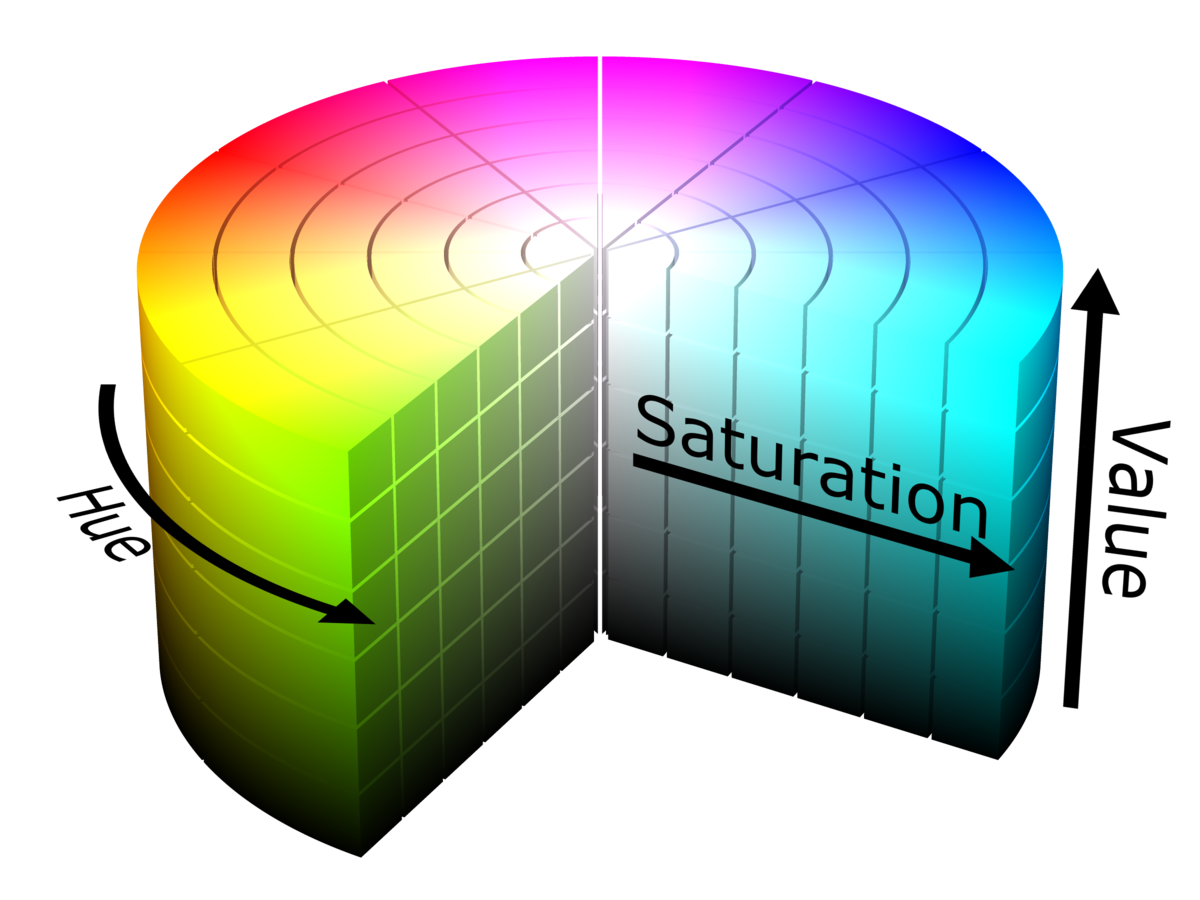
\includegraphics[width=0.5\textwidth]{hsv}
	\centering
	\caption[Representación del espacio de color HSV]{Representación del espacio de color HSV~\cite{wiki:hsv}.}
	\label{fig:hsv}
\end{figure}


\subsection{Puntos de la mano}
Una vez comprendidos los conceptos a la hora de procesar vídeos, viene el paso para obtener los puntos de la mano con los que extraer datos que sirvan para realizar una clasificación.

Mediante el objeto de lectura, se van extrayendo todos los fotogramas para procesarlos uno a uno. En cada fotograma, se dibujarán los puntos unidos mediante líneas con la biblioteca \textit{mediapipe} que se explica en el apartado de técnicas y herramientas~\ref{lib:mediapipe}, tal y como se aprecia en la figura~\ref{fig:puntosmano}. Sin embargo, en este trabajo, sólo serán importantes dos de ellos: el 4 y el 8, ya que son los que representan las puntas de los dedos pulgar e índice respectivamente.

\begin{figure}[h]
	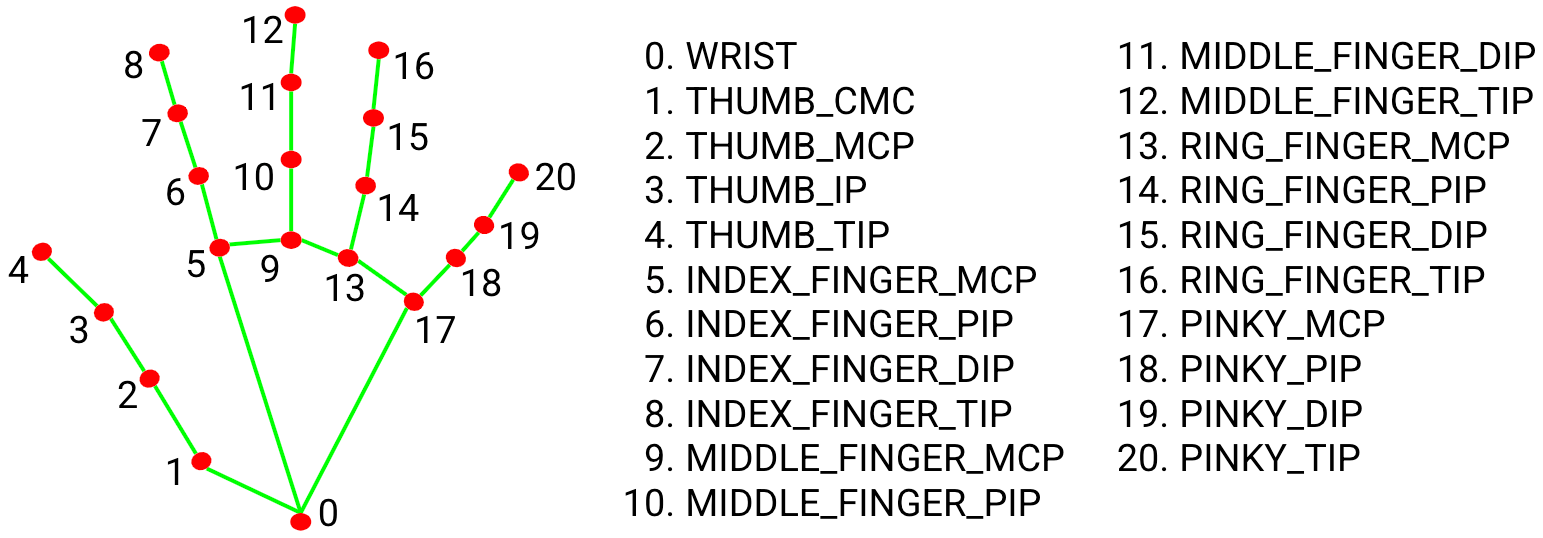
\includegraphics[width=1\textwidth]{puntos_mano}
	\centering
	\caption[Puntos de la mano y su nombre.]{Puntos de la mano y su nombre~\cite{mediapipehands}.}
	\label{fig:puntosmano}
\end{figure}

Una vez establecidos los puntos, se van a obtener las coordenadas de cada fotograma donde están ambos puntos, con el fin de obtener la distancia que los separa en cada instante.

\section{Limpieza de los datos} \label{limpieza}
Dado que la obtención de los datos del paso anterior no es perfecta, hay que utilizar alguna técnica para eliminar el posible ruido que la biblioteca ha podido ocasionar. Este ruido viene dado porque entre fotogramas, la biblioteca puede detectar el dedo en lugares diferentes sin que este se haya movido, provocando que la amplitud de la pinza se vea afectada.

\subsection{Filtro de Savitzky–Golay} \label{savgol}
Este filtrado~\cite{wiki:savgol} ha sido utilizado para eliminar algunas imperfecciones de los datos. Se basa en el cálculo de una regresión polinomial local de grado $k$ con al menos $k+1$ puntos equiespaciados que determinan el valor de un nuevo punto. Esto hará que los datos varíen y se suavice la gráfica. 

Al dibujar los datos en forma de gráfica, como se observa en la figura \ref{fig:graficadistancias}, se puede apreciar cómo algunas zonas no establecen un único máximo o el máximo podría estar exagerado, por lo que es necesario suavizar esos picos para obtener un solo máximo. 

\begin{figure}[h]
	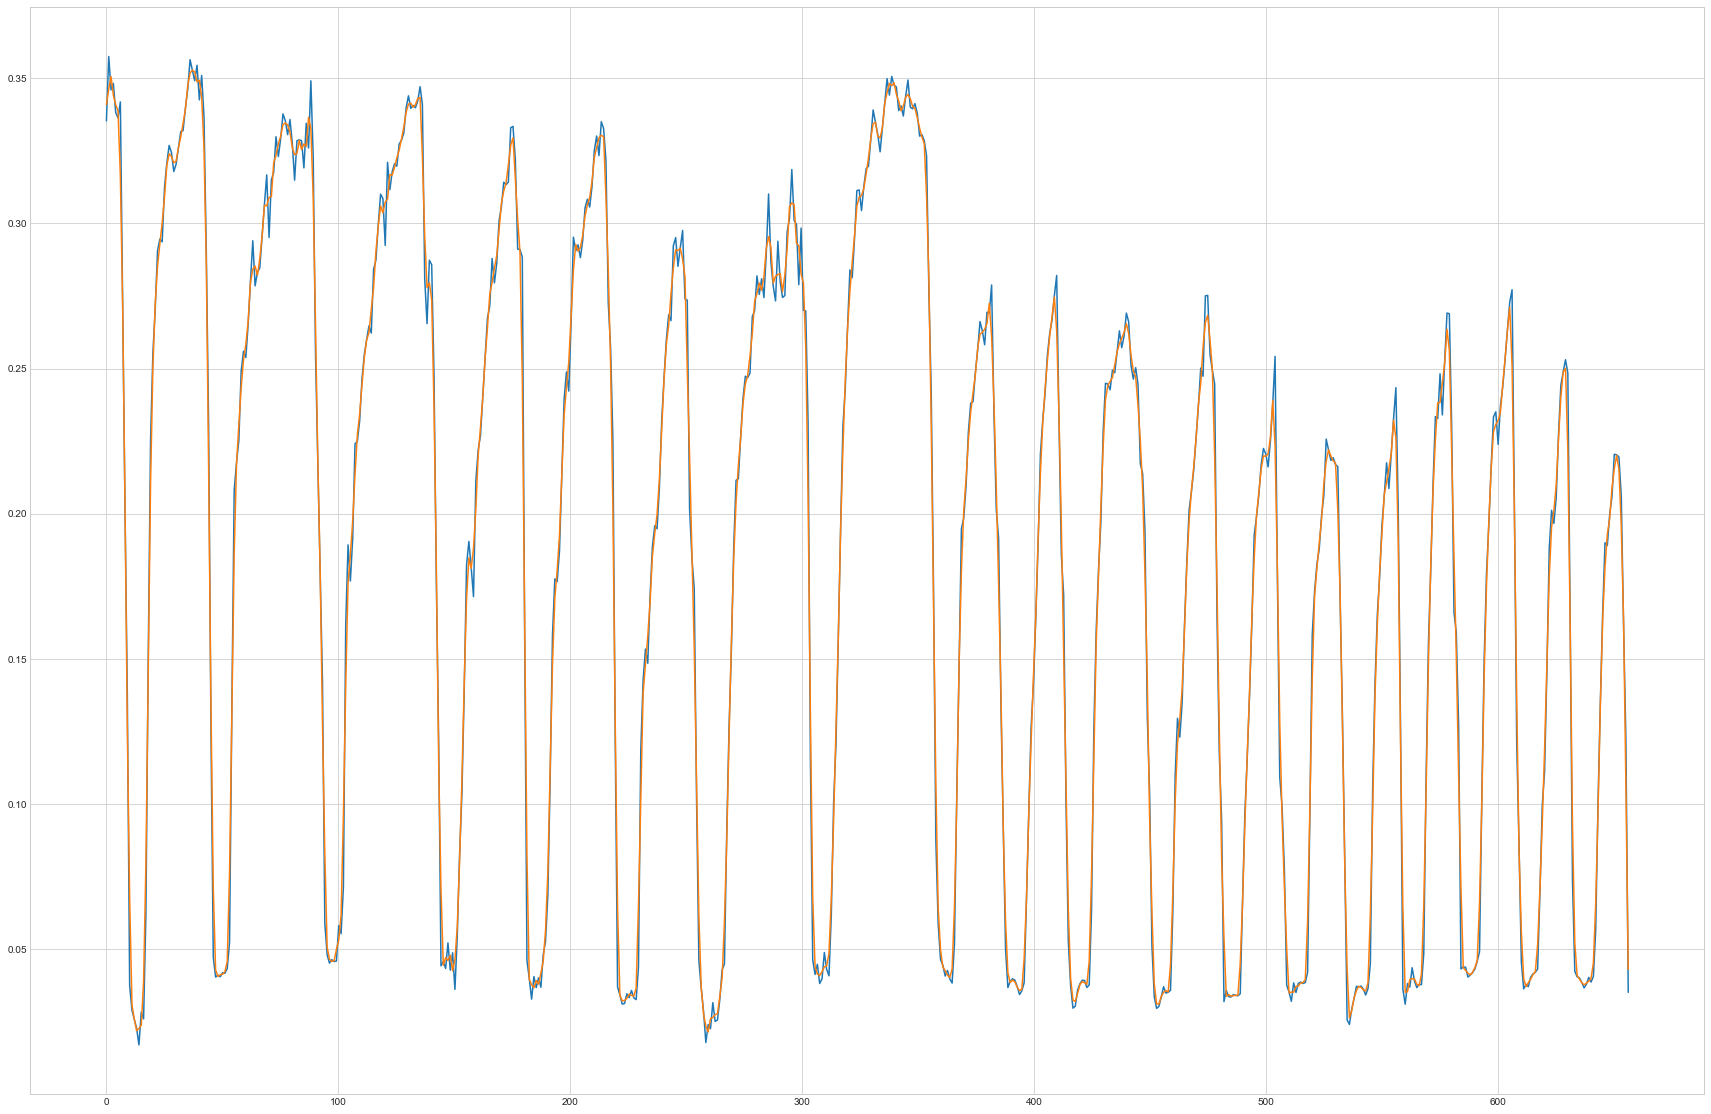
\includegraphics[width=1\textwidth]{grafica_distancias}
	\centering
	\caption[Representación gráfica de los datos obtenidos en uno de los vídeos con y sin filtrado.]{Representación gráfica de los datos obtenidos en uno de los vídeos sin filtrado (azul) y con filtrado (naranja).}
	\label{fig:graficadistancias}
\end{figure}

La figura \ref{fig:graficadistanciaszoom} muestra uno de los picos de forma ampliada, notándose el suavizado del filtro frente a la gráfica sin suavizar eliminando los picos que producen ruido. Lo ideal sería que la curva fuese lo más perfecta posible, pero el propio pulso de la mano y, sobre todo, la biblioteca que coloca los puntos sobre la mano provocan esas imperfecciones que conviene solucionar. No obstante, aun aplicando el filtrado, no se consigue el resultado ideal, pues el filtrado es únicamente una aproximación y una mejora del resultado real.

\begin{figure}[h]
	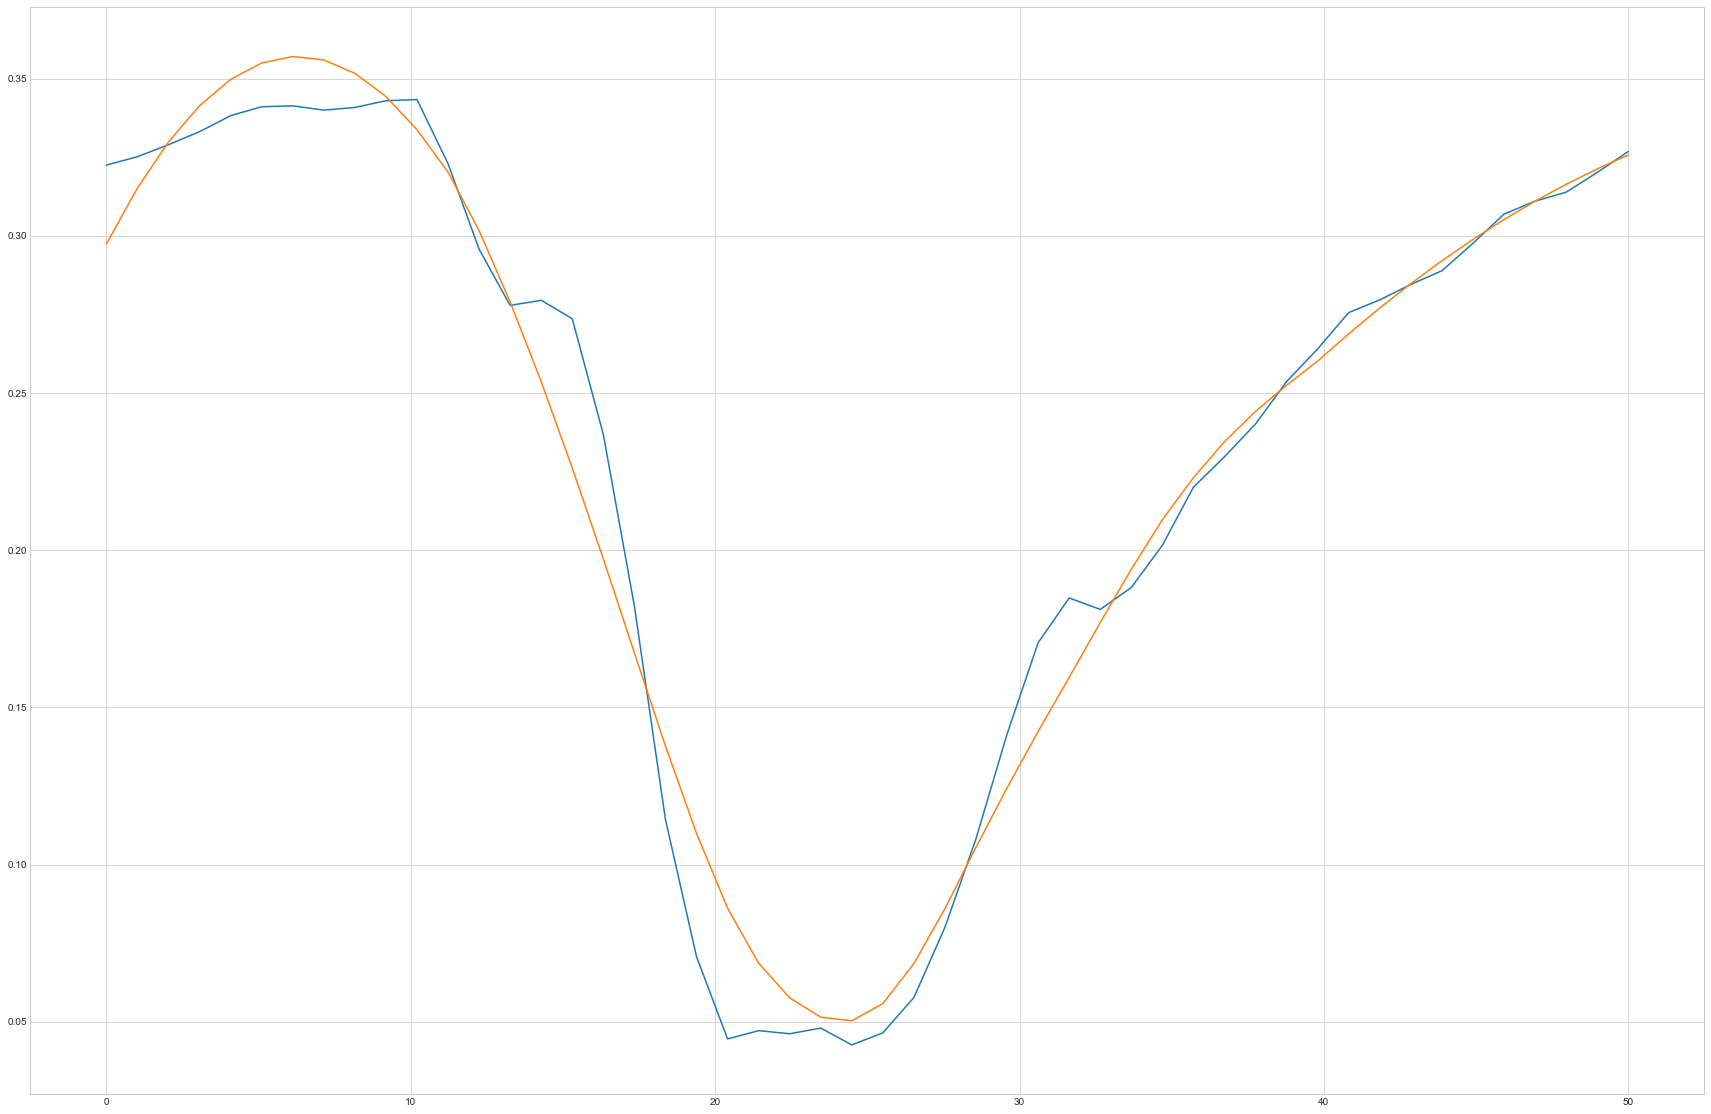
\includegraphics[width=1\textwidth]{grafica_distancias_zoom}
	\caption[Ampliación de uno de los picos donde se aprecia la curva con y sin suavizado.]{Ampliación de uno de los picos donde se aprecia la curva sin suavizar (azul) de la suavizada con el filtro (naranja).}
	\label{fig:graficadistanciaszoom}
\end{figure}

\section{Minería de datos}
Este punto trata de encontrar patrones en los datos que sirvan para clasificar. Para el problema planteado de predicción, hay que utilizar la clasificación.

La clasificación es una tarea de la minería de datos que realiza un proceso de asignación de una clase u otra dependiendo de los valores que tengan los datos. Extrapolado a este trabajo, esto sería asignar si una persona tiene Parkinson o no dependiendo de las características obtenidas en el punto anterior.

\subsection{Conjunto de ejemplos}
Las características obtenidas son las que conforman el conjunto de datos. Este conjunto de datos será mejor cuantos más ejemplos haya, ya que más opciones podrán abarcar los clasificadores y mejores serán las predicciones.

Los clasificadores se utilizan realizando una separación del conjunto total de los datos. Esta separación da lugar a los datos de entrenamiento y los datos de test:

\begin{itemize}
	\item Conjunto de entrenamiento: constituye la mayor parte de los datos, entre el 70 \% y 80 \% generalmente. Sirve para enseñar al modelo a clasificar el conjunto de datos, indicándole qué casos son de una clase y qué casos de otra.
	\item Conjunto de test: Sirve para probar cuánto de bueno es el modelo entrenado con los ejemplos de entrenamiento. Tras las predicciones, se comprobará la clase asignada a cada ejemplo y la clase real, para obtener unas precisiones.
\end{itemize}

El conjunto de entrenamiento ha de contener más ejemplos que el conjunto de test debido a que cuantos más ejemplos se ofrezcan al modelo, más probable es que aprenda correctamente. Además, para probar cómo de bueno es un modelo, no es necesario un alto número de ejemplos.

Es importante que a la hora de evaluar el modelo se utilicen datos que no han sido utilizados para entrenar el modelo, ya que esos ejemplos siempre los acertarían. Debido a esto, es necesario tener estas dos divisiones.

También es imprescindible que el conjunto de ejemplos esté equilibrado, es decir, que haya un equilibrio entre los ejemplos de una clase y de otra. Si un conjunto de datos no está equilibrado, al realizar el entrenamiento de un modelo, tenderá a predecir la clase mayoritaria. Además, si el número de ejemplos de la clase minoritaria es demasiado pequeño, el clasificador no tendrá suficientes ejemplos como para conocer cuándo se debe predecir esa clase, por lo que también conocerá más acerca de la clase mayoritaria y realizará las predicciones más a su favor.

\subsection{Validación cruzada}
La validación cruzada es una técnica que se utiliza a la hora de entrenar y probar modelos de aprendizaje. Se basa en dividir el conjunto de datos en un número de partes y utilizar cada una de las partes como conjunto de test y el resto para entrenar el modelo. Cada una de las partes será utilizada como conjunto de test de forma iterativa.

Con esto se consigue que la selección de los conjuntos de entrenamiento y test no perjudique al resultado del modelo y se puedan probar más posibilidades de división de los datos.

\subsection{Algoritmos de clasificación} \label{clasificadores}
Una de las formas más sencillas de encontrar patrones en los datos es utilizando modelos de aprendizaje. Hay varios modelos, y cada uno utiliza una forma de clasificar diferente. Los modelos empleados en este TFG son:
\begin{itemize}
	\item \textbf{Árboles de decisión:} se trata de construir un árbol formado por nodos con condiciones y hojas con clases, para que los datos sean clasificados dependiendo de si cumplen una condición de un nodo o no.~\cite{arbol_decision}
	\item \textbf{Random Forest:} se trata de clasificar los ejemplos utilizando varios árboles de decisión. Estos árboles se construyen utilizando un subconjunto del conjunto total de datos de entrenamiento. Cada árbol predecirá una clase, y la más frecuente será la que se le asigne al atributo.~\cite{random_forest}
	\item \textbf{k-Nearest Neighbors:} se trata de obtener la clase mayoritaria de los $k$ vecinos más cercanos al ejemplo que se trata de clasificar. En este clasificador, no hay un paso previo de entrenamiento, sino que se realiza la predicción utilizando el conjunto de entrenamiento original.~\cite{knn}
	\item \textbf{Naive Bayes:} se trata de calcular la frecuencia de aparición de los valores de cada característica para poder realizar una clasificación. Esto haría que un ejemplo con ciertos valores se le asigne una clase debido a la probabilidad de aparición de sus valores.~\cite{naive_bayes}
	\item \textbf{Naive Bayes Gaussiano:} es una variante del clasificador Naive Bayes y se trata de utilizar las probabilidades de que aparezcan los valores de los atributos, pero acorde con una distribución normal.~\cite{naive_bayes_g}
	\item \textbf{SVM:} se trata de conseguir un hiperplano que separe los ejemplos que compartan la misma clase del resto. A la hora de clasificar un ejemplo, dependiendo de dónde se encuentre, se le asignará una clase u otra.~\cite{svm}
	\item \textbf{Dummy:} es el clasificador más sencillo que existe, ya que siempre predice la clase que más veces aparece en el conjunto de datos, por lo que nunca tendrá buenas precisiones cuando los datos se encuentren equilibrados.~\cite{dummy}
\end{itemize}

\section{Evaluación de los resultados}
A la hora de evaluar los resultados, es importante realizar un estudio de los datos obtenidos para poder valorar correctamente los resultados.

\subsection{Predicciones}
Cuando se utiliza un clasificador, se realizan varias predicciones con el conjunto de test. En esta ocasión, hay dos clases posibles: sin Parkinson (0) o con Parkinson (1), por lo que pueden ocurrir cuatro posibilidades:

\begin{itemize}
	\item Verdadero positivo o \textit{true positive}: ocurre cuando una clase se predice correctamente y además es positiva. En este caso, sería que el clasificador ha predicho un 1 (positivo) y ha acertado. Suele indicarse como TP.
	\item Verdadero negativo o \textit{true negative}: ocurre cuando una clase se predice correctamente y además es negativa. En este caso, sería que el clasificador ha predicho un 0 (negativo) y ha acertado. Suele indicarse como TN.
	\item Falso positivo o \textit{false positive}: ocurre cuando una clase no se predice correctamente y además es positiva. En este caso, sería que el clasificador ha predicho un 1 (positivo) y ha fallado. Suele indicarse como FP.
	\item Falso negativo o \textit{false negative}: ocurre cuando una clase no se predice correctamente y además es negativa. En este caso, sería que el clasificador ha predicho un 0 (negativo) y ha fallado. Suele indicarse como FN.
	
\end{itemize}

\subsection{Medidas} \label{medidas}
Las medidas son formas de representar los resultados para obtener diferentes puntos de vista a la hora de evaluar los resultados. Las medidas utilizadas en este TFG son:

\begin{itemize}
	\item \textit{accuracy}: con esta medida se podrá obtener la precisión que ha tenido el clasificador. Esto es, el porcentaje de aciertos que ha habido. La fórmula que se utiliza es la siguiente:
	\begin{equation}
		accuracy = \frac{TP + TN}{TP + TN + FP + FN}
	\end{equation}

	\item \textit{Matthews correlation coefficient}: esta mediada es utilizada para conocer la calidad de una clasificación binaria. La fórmula para obtener esta medida es la siguiente:
	\begin{equation}
		MCC = \frac{TP\times TN-FP\times FN}{\sqrt{(TP+FP)\times(TP+FN)\times(TN+FP)\times(TN+FN)}}
	\end{equation}

	\item \textit{f1}: esta medida es utilizada para recoger las medidas de \textit{precision} y \textit{recall} en una sola medida. La medida \textit{precision} sirve para conocer los aciertos que ha habido en una clase concreta y la medida \textit{recall} sirve para conocer cuántos ejemplos han sido clasificados como una clase concreta. Estas fórmulas son las siguientes:
	\begin{align}
		precision &= \frac{TP}{TP+FP} &
		recall &= \frac{TP}{TP+FN}
	\end{align}
	
	Y la fórmula para obtener la medida f1 es la siguiente:
	\begin{equation}
		f1 = 2\times \frac{precision\times recall}{precision + recall}
	\end{equation}

	\item \textit{roc\_auc}: esta medida es el área bajo la curva ROC y representa cómo de bueno es un modelo a la hora de diferenciar una clase de otra. Dado que esta métrica es más complicada que las anteriores, más abajo se explica de forma más detallada.
	\item \textit{g\_mean}: esta medida es la media geométrica de la sensibilidad y la especificidad y trata de mostrar la precisión de las clases manteniendo las precisiones de forma equilibrada. Las fórmulas de sensibilidad y especificidad, se pueden ver más abajo. La fórmula para obtener esta medida es la siguiente:
	\begin{equation}
		g\_mean = \sqrt{sensibilidad \times especificidad}
	\end{equation}
\end{itemize}

\subsection{Curva ROC}
La curva ROC~\cite{wiki:roc} (\textit{Receiver Operating Characteristic}) es una representación gráfica utilizada para conocer la proporción de positivos bien clasificados y los positivos mal clasificados.

La curva ROC representada gráficamente tiene como eje $x$ la 1 $-$ especificidad y como eje $y$ la sensibilidad. La especificidad corresponde a los ejemplos negativos bien clasificados, o lo que es lo mismo, 1 menos los ejemplos positivos mal clasificados; y la sensibilidad corresponde a los ejemplos positivos bien clasificados. Sus correspondientes fórmulas son las siguientes:

\begin{align}
	especificidad &= \frac{TN}{FP+TN} &
	sensibilidad &= \frac{TP}{TP+FN}
\end{align}

Para dibujar la curva ROC habría que recoger varios resultados de un modelo y unir esos puntos para formar la curva, de forma que quede de forma similar que en la figura \ref{fig:roc}, en donde se visualizan tres tipos de curvas ROC que representan clasificaciones de mejor a peor.

\begin{figure}[h]
	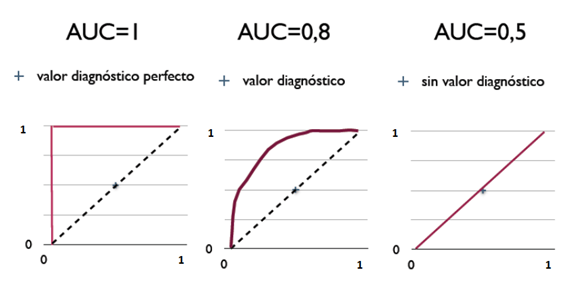
\includegraphics[width=1\textwidth]{curvas_roc}
	\caption[Tres tipos de curvas ROC.]{Tres tipos de curvas ROC~\cite{wiki:roc}.}
	\label{fig:roc}
\end{figure}

\subsection{Área bajo la curva ROC}
El área bajo la curva ROC (\textit{Area Under the ROC Curve}) es la medida con la que conocer cómo de bien un modelo diferencia una clase de otra.

Este área no es más que el cálculo de todo el área que hay debajo de la curva ROC. Los valores obtenidos estarán en el intervalo [0,1]. Los valores comprendidos entre 0 y 0,5 indican que el modelo confunde una clase con otra en su mayor parte, mientras que los valores comprendidos entre 0,5 y 1 indican que el modelo predice correctamente la mayoría de ejemplos, siendo el valor 1 la perfección. En la figura \ref{fig:roc} se aprecian tres valores AUC para cada curva, mostrando que la primera trata de un clasificador perfecto mientras que la última muestra un clasificador mucho peor.
